\documentclass{ceurart}

\usepackage{booktabs}
\usepackage{enumitem}
\usepackage{amsmath}
\usepackage{xcolor}
\usepackage{siunitx}
\usepackage{tabularx}
\usepackage{adjustbox}
\usepackage{tikz}
\usetikzlibrary{arrows.meta,positioning,fit}

\sloppy

\newcommand{\dataset}[1]{\texttt{#1}}
\newcommand{\method}[1]{\texttt{#1}}
\newcommand{\datasetname}[1]{\mbox{\texttt{\small #1}}}
\newcolumntype{Y}{>{\raggedright\arraybackslash}X}

\copyrightyear{2026}
\copyrightclause{Copyright for this paper by its authors.
  Use permitted under Creative Commons License Attribution 4.0
  International (CC BY 4.0).}

\conference{CLEF 2026 Working Notes, September 21--24, 2026, Jena, Germany}

\title{Dataset-Routed Clustering with Candidate Pair Constraints for AnimalCLEF 2026}
\author[1,2]{Yaokai Ge}[%
email=geyk886@163.com,
]
\author[1,2]{Mingshun Zhu}[%
email=22009200471@stu.xidian.edu.cn,
]
\author[1,2]{Chen He}[%
email=hechen@ict.ac.cn,
orcid=0000-0003-0124-8860,
]
\author[1,2]{Ruiping Wang}[%
email=wangruiping@ict.ac.cn,
orcid=0000-0003-1830-2595,
]

\address[1]{Key Laboratory of AI Safety of Chinese Academy of Sciences (CAS), Institute of Computing Technology, CAS, Beijing, 100190, China}
\address[2]{University of Chinese Academy of Sciences, Beijing, 100049, China}

\begin{document}

\begin{abstract}
AnimalCLEF 2026 evaluates individual animal discovery and re-identification as an open-set clustering task across four dataset namespaces: \dataset{LynxID2025}, \dataset{SalamanderID2025}, \dataset{SeaTurtleID2022}, and \dataset{TexasHornedLizards}. Each test image must be assigned to an identity cluster and submissions are evaluated using Adjusted Rand Index. We describe a dataset-routed clustering pipeline that combines foundation wildlife descriptors, supervised metric-learning heads, local feature evidence, learned pairwise fusion, transductive smoothing, and candidate pair constraints. The core idea is to decompose clustering into two stages: a high-recall automatic stage that retrieves top-$K$ candidate links, followed by a precision-oriented pair-constraint stage that turns ambiguous candidates into graph constraints. This strategy was first developed for \dataset{TexasHornedLizards}, where the official Texas horned lizard study motivated ventral-pattern preprocessing and local matching, and was later reused for \dataset{SalamanderID2025}. Our final submission obtained 0.67987 public ARI and 0.69632 private ARI in the AnimalCLEF 2026 competition.
\end{abstract}

\begin{keywords}
animal re-identification \sep
open-set clustering \sep
metric learning
\end{keywords}

\maketitle

\section{Introduction}
Individual animal re-identification aims to recognise the same animal across photographs collected at different times, locations, viewpoints, and acquisition conditions. It is an important tool for ecological monitoring because many species can be identified from persistent visual markings such as coat patterns, scales, scutes, stripes, spots, or ventral markings. Compared with human re-identification, animal re-identification is often more open-ended: the number of individuals is not fixed, many individuals have only a few images, backgrounds and camera traps can be highly biased, and the visual cue differs substantially across species \cite{schneider2019animalreid,wildlifedatasets}.

AnimalCLEF 2026, organised within LifeCLEF 2026, casts this general problem as discovery-oriented clustering across four animal datasets \cite{lifeclef2026,animalclef2026overview}. This setting makes the objective different from ordinary retrieval: a model with high nearest-neighbour recall can still fail if its clustering threshold merges different individuals, while a conservative pipeline can fail by over-splitting the same animal. The official metric is Adjusted Rand Index (ARI), a chance-corrected measure of agreement between two partitions \cite{hubert1985comparing}.

Our final pipeline was built around one observation: the four datasets expose different visual and statistical structures, so a single backbone and threshold is not robust. Lynx images contain relatively stable coat patterns and strong cluster-count priors. Salamanders require fine local texture and careful ambiguity handling. Sea turtles are already well served by frozen wildlife descriptors. Texas horned lizards have no labelled local train split in the released package, making them a strong domain-shift and self-training problem. We therefore use a dataset-routed pipeline in which each species branch has its own representation, pair evidence, thresholding, and post-processing policy.

The key simplification is to avoid treating clustering as one monolithic thresholding problem. We instead split it into a high-recall first stage and a precision-oriented second stage. The first stage is allowed to be inclusive: global descriptors, local ORB evidence, and species-specific preprocessing only need to surface plausible same-individual links. The second stage is selective: candidate pair verification converts a much smaller ambiguity set into positive and negative graph constraints.

The verification component of our pipeline was inspired by ambiguity-aware pair sampling for animal re-identification \cite{sani2026active}. That work frames feedback as pairwise constraints, producing must-link and cannot-link signals for constrained clustering. We adopt the same pairwise interface in a narrower engineering form: the model proposes candidate pairs, and the verification stage only accepts or rejects pair edges. In our competition setting, these decisions are compiled into clustering constraints over top-$K$ local matches and uncertain clusters.

Our contributions are:
\begin{itemize}[leftmargin=*]
  \item A practical dataset-routed clustering pipeline for AnimalCLEF 2026, with official scores of 0.67987 public ARI and 0.69632 private ARI.
  \item A two-stage clustering decomposition that uses automatic top-$K$ candidate retrieval for recall and pair-constraint verification for precision.
  \item An account of the species-specific routes that proved useful: transductive seed smoothing for lynx, learned pairwise fusion and graph constraints for salamanders, conservative descriptor fusion for sea turtles, and trusted-view self-training for Texas horned lizards.
  \item Documented intervention evidence showing that many useful components were not universal: ORB local matching helped salamanders but was not used for lynx or sea turtles, yellow-pattern cues hurt as hard vetoes but helped as learned XGBoost features, and Texas descriptor concatenation degraded despite preserving seed pairs.
\end{itemize}

\section{Related Work}
\subsection{Animal Re-Identification}
Animal re-identification has historically relied on species-specific visual cues and semi-automatic photo-identification tools, especially for animals with stable markings \cite{schneider2019animalreid}. Recent benchmarks and toolkits have made the setting more comparable across species. WildlifeDatasets collects many individual animal datasets and provides a common evaluation interface, and MegaDescriptor is one of the strongest general descriptors from this line of work \cite{wildlifedatasets}. MiewID is another multispecies model trained from community-curated identity data and was complementary to MegaDescriptor in our experiments \cite{miewid}. Dataset-specific benchmarks are also important: SeaTurtleID2022 emphasizes long-span open-set re-identification under realistic temporal splits \cite{seaturtleid2022}, while CzechLynx provides a large camera-trap resource for Eurasian lynx individual identification and related vision tasks \cite{czechlynx}.

\subsection{Local Matching and Species-Specific Cues}
Local feature matching is useful when identity is encoded in spatially localized markings. ORB provides a fast binary keypoint descriptor that can be paired with geometric verification \cite{orb}, while modern matchers such as LightGlue offer stronger learned correspondences for image matching \cite{lightglue}. For Texas horned lizards, the official reference study by Biffi et al. showed that ventral spot patterns carry individual identity information: HotSpotter placed the correct previous image first for 85 of 90 known recapture photos, and in four additional cases the correct match was still among the top-10 recommendations \cite{biffi2025identification}. This supports a useful separation between local matching as candidate retrieval and later decisions about which candidate links are reliable.

\subsection{Constrained Clustering and Pair Feedback}
Open-set re-identification pipelines often need to convert retrieval evidence into a partition, so pair-level decisions become useful when descriptor scores alone are ambiguous. Ambiguity-aware pair sampling for animal re-identification converts selected pairwise feedback into must-link and cannot-link constraints for clustering \cite{sani2026active}. We use this line of work as the conceptual basis for treating verified candidate pairs as graph constraints.

\section{Task and Data}
\subsection{Task Definition}
The goal of AnimalCLEF 2026 is to discover individual animals in the hidden test split and submit the resulting identity partition. In other words, participants are not asked to predict species labels or to assign images to a fixed set of known training identities. They must group the unlabelled test images so that photographs of the same animal receive the same cluster identifier and photographs of different animals receive different identifiers.

The input consists of four dataset namespaces, labelled training identities where available, and unlabelled test images. The required submission is a CSV file with two columns, \method{image\_id} and \method{cluster}. The official evaluation compares the submitted partition with the hidden ground-truth identity partition using Adjusted Rand Index (ARI). We therefore treat AnimalCLEF 2026 as an open-set clustering task, where retrieval scores are only intermediate evidence and the final object being evaluated is the complete test-set clustering.

\subsection{Dataset Splits}

The officially released data contain 15,483 images in four dataset namespaces. The train split contains 13,074 labelled images for three datasets, while \datasetname{TexasHornedLizards} is provided as a test-only dataset with 274 images. The test split contains 2,409 images in total. The datasets are released through the AnimalCLEF benchmark \cite{animalclef2026overview}; where available, we also cite the underlying dataset or species study used by the benchmark \cite{animalclef2025overview,seaturtleid2022,czechlynx,biffi2025identification}.

\begin{table}[t]
  \centering
  \caption{Dataset sizes in the released AnimalCLEF 2026 package used by our pipeline.}
  \label{tab:data}
  \begin{tabular}{lrrl}
    \toprule
    Dataset & Train images & Test images & Main visual cue / source \\
    \midrule
    \dataset{LynxID2025} & 2,957 & 946 & coat/flank markings; CzechLynx-related \cite{czechlynx} \\
    \dataset{SalamanderID2025} & 1,388 & 689 & dorsal yellow spot patterns \cite{animalclef2025overview} \\
    \dataset{SeaTurtleID2022} & 8,729 & 500 & facial and scute patterns \cite{seaturtleid2022} \\
    \dataset{TexasHornedLizards} & 0 & 274 & ventral/body spot patterns \cite{biffi2025identification} \\
    \midrule
    Total & 13,074 & 2,409 & -- \\
    \bottomrule
  \end{tabular}
\end{table}

The labelled train distribution is strongly long-tailed. Across the three labelled datasets there are 1,102 identities and 317 singleton identities. Salamander is the most extreme case: \dataset{SalamanderID2025} has 587 train identities, of which about 52.8\% are singletons. This matters because identity-level validation and pairwise training produce very different support across datasets. Figure~\ref{fig:identity-distribution} shows the per-dataset identity-size distribution that motivated the dataset-routed design.

\begin{figure}[t]
  \centering
  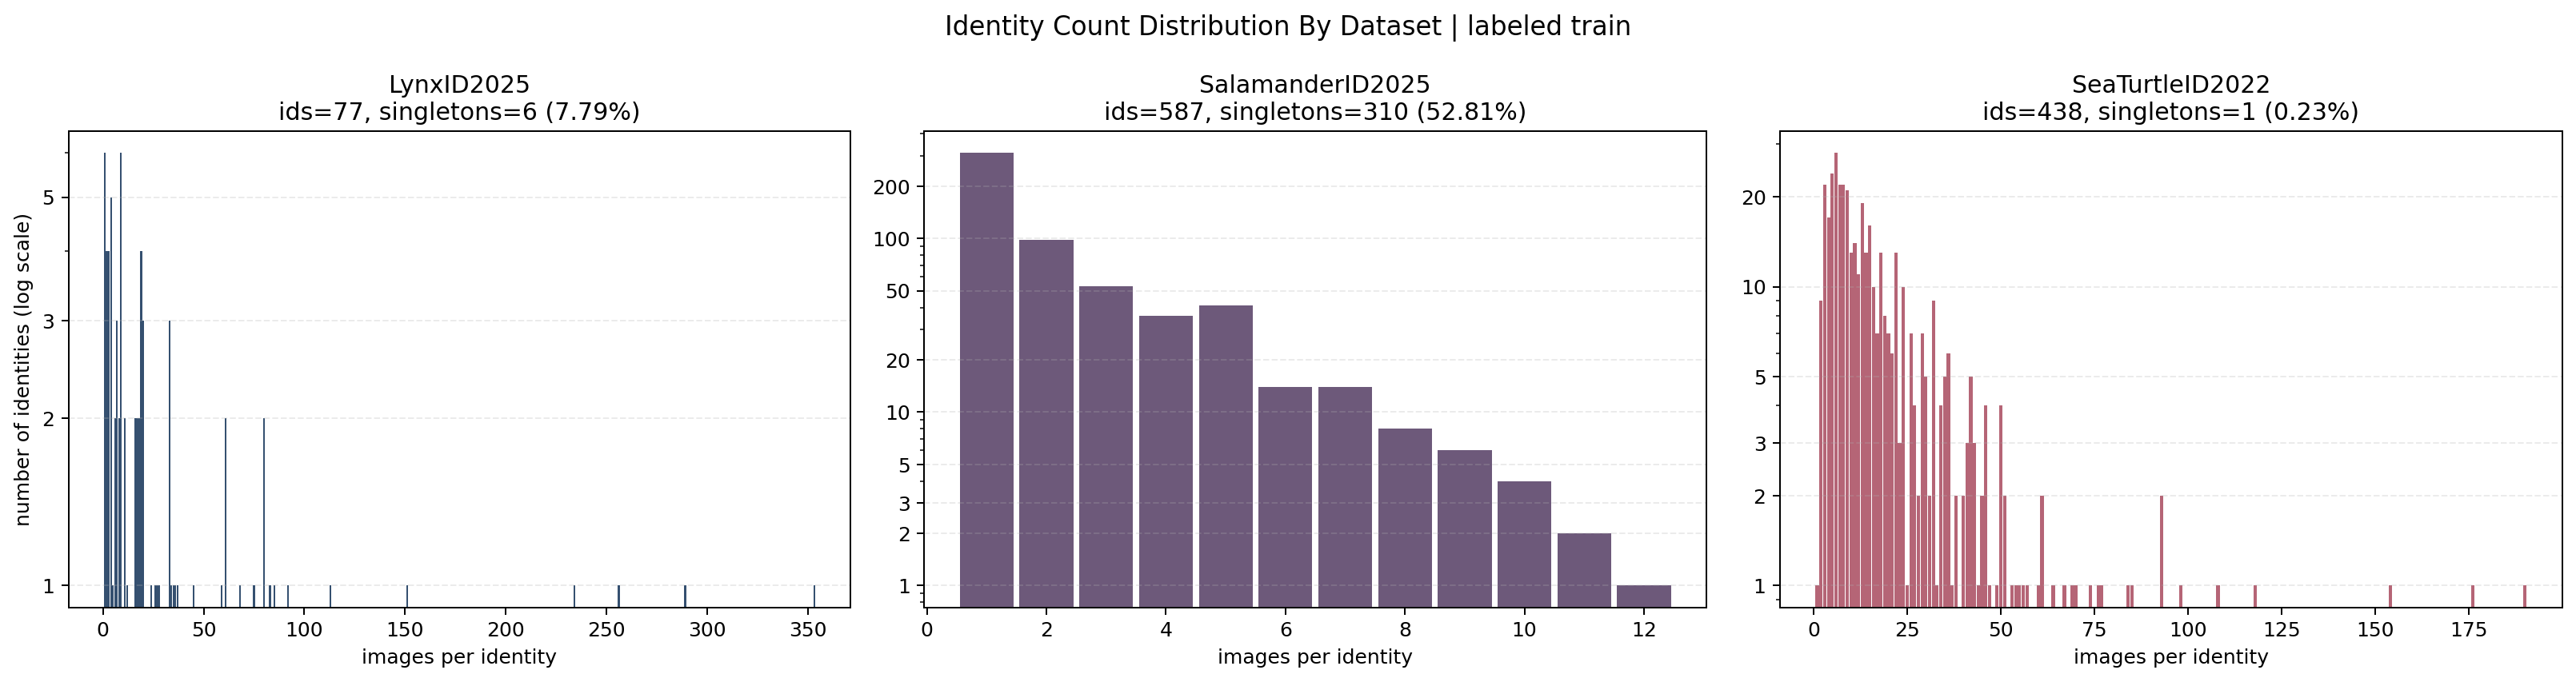
\includegraphics[width=\linewidth]{figures/identity_distribution_by_dataset.png}
  \caption{Identity-size distribution in the labelled training split. Salamander is dominated by singleton identities, while sea turtle has many multi-image identities and lynx has fewer identities with a long-tailed image count. This motivates identity-level validation and species-specific clustering policies.}
  \label{fig:identity-distribution}
\end{figure}

\paragraph{Local validation protocol.}
Local validation refers to our internal experiment protocol, not the official Kaggle evaluation split. For each labelled dataset, identities are shuffled with seed 42 and approximately 10\% of identities are held out; all images of the same individual stay on the same side of the split. This produces 991 fit identities with 11,739 fit images and 111 validation identities with 1,335 validation images. The validation split contains 69/8 fit/validation identities for lynx, 528/59 for salamander, and 394/44 for sea turtle. Official competition scores are reported separately from the Kaggle public and private leaderboards.

We report ARI as the main clustering metric. We also track Normalized Mutual Information, pairwise precision/recall/F1, Recall@1/5/10, cluster count, and singleton-cluster ratio. Retrieval metrics are treated only as candidate-recall diagnostics: a high Recall@10 means that the global route can supply useful candidates, but the final objective remains the ARI of the cluster partition.

\section{Pipeline Overview}
Figure~\ref{fig:overview} summarises the pipeline. Each image is routed by dataset. Most branches start from two pretrained wildlife descriptors: MiewID \cite{miewid} and MegaDescriptor \cite{wildlifedatasets}. We use cosine similarity on L2-normalised embeddings, average-linkage clustering for descriptor-only routes, and graph-style post-processing where pairwise evidence is more reliable than global thresholds.

\begin{figure}[ht]
  \centering
  \begin{adjustbox}{max width=\linewidth}
  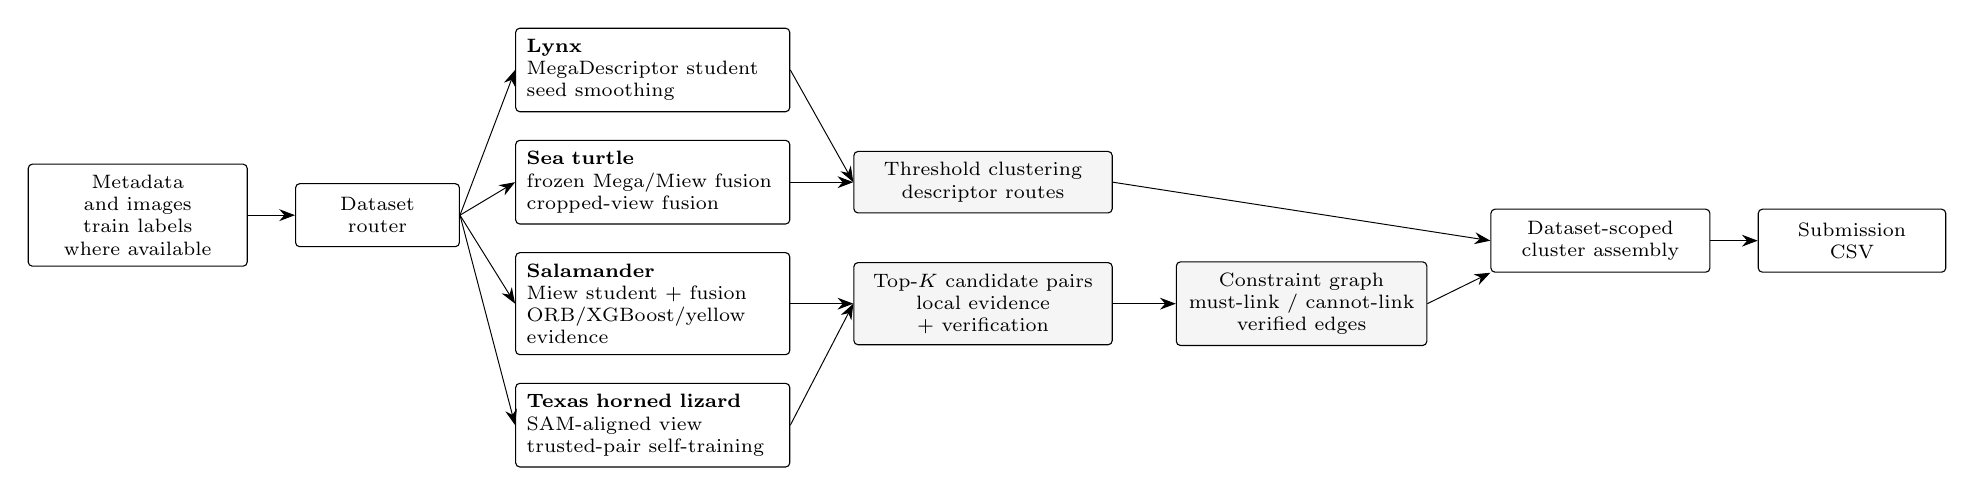
\begin{tikzpicture}[
    font=\scriptsize,
    node distance=3.5mm and 6mm,
    block/.style={draw, rounded corners=1.5pt, align=center, inner sep=4pt, minimum height=8mm},
    route/.style={draw, rounded corners=1.5pt, align=left, inner sep=4pt, text width=32mm},
    stage/.style={draw, rounded corners=1.5pt, align=center, inner sep=4pt, fill=gray!8},
    arrow/.style={-{Stealth[length=2mm]}, line width=0.35pt}
  ]
    \node[block, text width=25mm] (input) {Metadata and images\\train labels where available};
    \node[block, right=of input, text width=18mm] (router) {Dataset\\router};
    \node[route, above right=9mm and 7mm of router] (lynx) {\textbf{Lynx}\\MegaDescriptor student\\seed smoothing};
    \node[route, below=of lynx] (turtle) {\textbf{Sea turtle}\\frozen Mega/Miew fusion\\cropped-view fusion};
    \node[route, below=of turtle] (salamander) {\textbf{Salamander}\\Miew student + fusion\\ORB/XGBoost/yellow evidence};
    \node[route, below=of salamander] (texas) {\textbf{Texas horned lizard}\\SAM-aligned view\\trusted-pair self-training};
    \node[stage, right=8mm of turtle, text width=30mm] (threshold) {Threshold clustering\\descriptor routes};
    \node[stage, right=8mm of salamander, text width=30mm] (pairs) {Top-$K$ candidate pairs\\local evidence + verification};
    \node[stage, right=8mm of pairs, text width=29mm] (graph) {Constraint graph\\must-link / cannot-link\\verified edges};
    \node[block, right=8mm of graph, yshift=8mm, text width=25mm] (assembly) {Dataset-scoped\\cluster assembly};
    \node[block, right=of assembly, text width=21mm] (output) {Submission\\CSV};

    \draw[arrow] (input) -- (router);
    \draw[arrow] (router.east) -- (lynx.west);
    \draw[arrow] (router.east) -- (salamander.west);
    \draw[arrow] (router.east) -- (turtle.west);
    \draw[arrow] (router.east) -- (texas.west);
    \draw[arrow] (lynx.east) -- (threshold.west);
    \draw[arrow] (turtle.east) -- (threshold.west);
    \draw[arrow] (salamander.east) -- (pairs.west);
    \draw[arrow] (texas.east) -- (pairs.west);
    \draw[arrow] (pairs) -- (graph);
    \draw[arrow] (threshold.east) -- (assembly.west);
    \draw[arrow] (graph.east) -- (assembly.south west);
    \draw[arrow] (assembly) -- (output);
  \end{tikzpicture}
  \end{adjustbox}
  \caption{Pipeline overview. Images are first routed by dataset. Lynx and sea turtle use descriptor-based threshold clustering, while salamander and Texas horned lizard use high-recall top-$K$ candidate pairs followed by pair verification and constraint-graph compilation. The dataset-scoped cluster outputs are then assembled into the submitted CSV.}
  \label{fig:overview}
\end{figure}

For a descriptor matrix $E$ with L2-normalised rows, the base similarity is
\begin{equation}
  s(i,j)=E_i^\top E_j .
\end{equation}
Here $E_i$ and $E_j$ denote the embeddings of images $i$ and $j$, and $s(i,j)$ is their cosine similarity because each row of $E$ is L2-normalised.
For frozen descriptor fusion, MegaDescriptor and MiewID embeddings are concatenated and L2-normalised. For learned routes, a supervised student projects the backbone output into a 512-dimensional embedding and is clustered using a dataset-specific threshold.

The descriptor-only clustering route uses cosine distance followed by average-linkage hierarchical clustering implemented with scikit-learn \cite{scikit-learn}. Each dataset is clustered independently, and thresholds are swept on validation where labels are available. The submitted labels are dataset-scoped cluster strings that preserve the row order and schema of the sample submission. Detailed branch configurations and operating parameters are reported in Appendix~\ref{app:implementation-details}.

\begin{table}[t]
  \centering
  \caption{Final submission recipe by dataset.}
  \label{tab:final-recipe}
  \small
  \begin{tabularx}{\linewidth}{lYl}
    \toprule
    Dataset & Final route & Cluster policy \\
    \midrule
    \dataset{LynxID2025} & MegaDescriptor-L supervised student with transductive seed smoothing & average-linkage thresholding \\
    \dataset{SalamanderID2025} & MiewID student, frozen descriptor fusion, ORB evidence, yellow-pattern features, and XGBoost pair scoring & graph constraints over candidate pairs \\
    \dataset{SeaTurtleID2022} & frozen MegaDescriptor+MiewID fusion with a cropped-view fusion branch & conservative average-linkage thresholding \\
    \dataset{TexasHornedLizards} & SAM-aligned gray center-body views and trusted-view MiewID self-training & thresholding plus candidate-pair graph repair \\
    \bottomrule
  \end{tabularx}
\end{table}

\paragraph{Two-stage candidate pair verification.}
We use candidate pair verification as a narrow, operational form of ambiguity-aware pair sampling. Here verification means a same-individual or different-individual decision for a retrieved image pair. It can be produced by automatic confidence rules, by a learned pair scorer, or by explicit pair review; it is not inherently a manual labelling stage. The clustering problem is decomposed into a high-recall candidate-link stage and a precision-oriented verification stage. The pipeline does not assign global identity labels to arbitrary images. Instead, it repeatedly constructs a candidate set of image pairs:
\begin{enumerate}[leftmargin=*]
  \item Preprocess images into a view that exposes the relevant individual markings.
  \item Use descriptors and local matching to retrieve top-$K$ high-recall candidate pairs.
  \item Verify only these candidate pairs, either through automatic confidence rules or explicit pair review.
  \item Convert verified pair decisions into must-link, cannot-link, split, or attach constraints.
  \item Recompile the clustering graph using these constraints.
\end{enumerate}
The verification interface only exposes model-selected image pairs from the released competition data and produces pair-level graph evidence. For a dataset with $n$ images and $K$ retrieved neighbours per query, this reduces the candidate space from arbitrary all-pairs comparison to an $nK$ retrieval proxy; in our main runs $K=10$.
This design separates recall and precision. The automatic first stage only needs to avoid missing plausible same-individual pairs, so it can use inclusive top-$K$ retrieval and local matching. The second stage filters those candidates into high-precision evidence. In early Texas experiments this second stage was implemented with automatic trusted-pair rules; later versions used explicit pair review for the most ambiguous links. This is especially useful in AnimalCLEF 2026 because the official output is a clustering, and pair constraints map naturally onto cluster merges and splits: if retrieval is strong enough to surface the correct neighbours, verified pair edges can serve as a compact proxy for the desired cluster structure.

\section{Representation Learning and Pair Evidence}
\subsection{Foundation Descriptors}
Our first baselines used frozen MiewID-msv3 and MegaDescriptor-L embeddings. Both embeddings are L2-normalised, concatenated for early fusion, and normalised again. The two descriptors were complementary: MiewID was stronger than MegaDescriptor on salamanders, while MegaDescriptor was stronger on sea turtles. Their early fusion was the strongest no-training baseline on all three labelled validation datasets, as shown in Table~\ref{tab:baselines}.

\begin{table}[t]
  \centering
  \caption{Identity-level validation ARI for frozen descriptor baselines. Texas is excluded because no labelled train split is available locally.}
  \label{tab:baselines}
  \begin{tabular}{lrrr}
    \toprule
    Route & Lynx ARI & Salamander ARI & SeaTurtle ARI \\
    \midrule
    Frozen MiewID & 0.0864 & 0.1681 & 0.7854 \\
    Frozen MegaDescriptor & 0.1027 & 0.1078 & 0.8903 \\
    Frozen MegaDescriptor + MiewID & 0.2250 & 0.2030 & 0.9256 \\
    \bottomrule
  \end{tabular}
\end{table}

\subsection{Supervised Metric Learning}
We fine-tuned MiewID- and MegaDescriptor-initialised models on the labelled train splits of lynx, salamander, and sea turtle using separate metric-learning classification heads for each labelled dataset. Across repeated stable retraining runs, Mega-initialised routes were strongest for lynx, while Miew-initialised routes were more useful for salamanders. Sea turtle did not consistently benefit from fine-tuning over frozen fusion. Additional training details are given in Appendix~\ref{app:implementation-details}.

\subsection{Local Matching}
For salamanders and Texas horned lizards, whole-image descriptors were not enough. We therefore used ORB keypoint matches \cite{orb} with RANSAC geometric verification \cite{ransac} on top-$K$ candidate neighbours. The local score is used as a conservative boost or pair feature rather than as a full replacement for global similarity. This gate improved salamander validation ARI from 0.2030 to 0.2940, while smoke tests did not justify enabling it for lynx or sea turtle. Exact matching parameters are listed in Appendix~\ref{app:implementation-details}.

\subsection{XGBoost Pairwise Fusion}
The final salamander branch treats clustering as pairwise edge selection. We train an XGBoost classifier \cite{xgboost} on labelled salamander pairs and apply it to candidate test pairs. Features include route similarities, supervised-student similarity, frozen descriptor fusion similarity, ORB local evidence, and later yellow-pattern features extracted from SAM-masked views \cite{sam}. Candidate pairs whose predicted score passes the selected threshold become merge edges; connected components and graph-constraint overlays then form final clusters.

\subsection{Curated Constraint Compilation}
The pair verification output is compiled as graph constraints rather than directly edited labels. Verified positive pairs become high-priority must-link edges. Verified negative pairs become cannot-link constraints. Within a candidate cluster, edges are considered in descending priority: verified positive edges first, then model-scored edges whose XGBoost probability exceeds the graph threshold. A union operation is allowed only if it does not place a cannot-link pair in the same component.

Algorithm~1 summarizes the graph compiler. The procedure treats verified and model-scored pair evidence as ordered graph edges. Its only non-standard operation is \textsc{Compatible}: before a merge is committed, the algorithm checks a dynamic forbidden-neighbour map so that cannot-link constraints are propagated after every component merge.

\begin{center}
\begin{minipage}{0.96\linewidth}
\small
\begin{tabularx}{\linewidth}{@{}rX@{}}
\toprule
\multicolumn{2}{@{}l}{\textbf{Algorithm 1. Constrained pair-graph compilation}} \\
\midrule
\textbf{Require} &
base partition $C_0$; scored candidate pairs $P=\{(i,j,p_{ij})\}$; verified must-links $M$; verified cannot-links $N$; graph threshold $\tau$. \\
\textbf{Ensure} &
final partition $C$. \\
\midrule
1 &
$U \leftarrow$ disjoint-set over all test images. \\
2 &
For every cluster $S \in C_0$, union all images in $S$ in $U$. \\
3 &
For each current component $A$, initialise $F[A]\leftarrow\emptyset$. For every $(a,b)\in N$, add $\mathrm{find}_U(b)$ to $F[\mathrm{find}_U(a)]$ and add $\mathrm{find}_U(a)$ to $F[\mathrm{find}_U(b)]$. \\
4 &
$E_M \leftarrow [(i,j,1):(i,j)\in M]$ and $E_P \leftarrow \mathrm{sort}_{\mathrm{desc}}\{(i,j,p_{ij})\in P:p_{ij}\geq\tau\}$ by score $p_{ij}$; set $E \leftarrow E_M \,\Vert\, E_P$. \\
5 &
\textbf{for} each $(i,j,s)\in E$ \textbf{do} \\
6 &
\quad $A \leftarrow \mathrm{find}_U(i)$, $B \leftarrow \mathrm{find}_U(j)$. \\
7 &
\quad \textbf{if} $A=B$ \textbf{then} continue. \\
8 &
\quad \textbf{if} \textsc{Compatible}$(A,B,F)$ \textbf{then} \\
9 &
\quad\quad $R\leftarrow$ union$(A,B)$; set $F[R]\leftarrow(F[A]\cup F[B])\setminus\{A,B\}$. \\
10 &
\quad\quad Replace every occurrence of $A$ or $B$ in the remaining forbidden sets by $R$. \\
11 &
\quad \textbf{else} discard $(i,j,s)$ as a conflicting edge. \\
12 &
\textbf{end for} \\
13 &
$C \leftarrow$ connected components induced by $U$. \\
14 &
Apply deterministic split and anchor-attachment overlays, and return $C$. \\
\bottomrule
\end{tabularx}
\end{minipage}
\end{center}

This makes the constraint layer a controlled repair stage rather than an unbounded fragmentation step. Compiler thresholds and overlay counts are moved to Appendix~\ref{app:implementation-details}.

\section{Species-Specific Routes}
\subsection{LynxID2025}
Lynx images have stable coat patterns and a relatively small number of identities compared with the test image count. We therefore used a supervised MegaDescriptor route as the base, then applied transductive seed smoothing. Stable high-confidence seed clusters define centroids, and embeddings close to a seed centroid are moved toward that centroid before threshold clustering. On local validation, seed smoothing improved ARI from 0.4937 to 0.5625. A single-factor official submission also improved the public leaderboard from 0.48524 to 0.48670, with a later alpha setting reaching 0.48755.
Additional co-association probes are summarized in Appendix~\ref{app:route-details}.

\subsection{SalamanderID2025}
Salamander was the most engineering-heavy branch because global descriptors alone did not reliably resolve local yellow-pattern ambiguity. The branch therefore converted retrieval into pair evidence: descriptors and ORB local matching supplied high-recall candidate pairs, while XGBoost and graph constraints selected which local evidence should become cluster edges. After the Texas horned lizard branch showed that local top-$K$ retrieval plus pair-constraint verification could produce high-value trusted evidence, we reused the same workflow for salamanders. The visible identity cue changes from ventral lizard spots to dorsal yellow spot patterns, so the final branch combined frozen descriptor fusion, a supervised MiewID-based student, ORB local evidence, XGBoost pairwise fusion, yellow-pattern features, and graph constraints. ORB itself detects grayscale keypoints and does not know which structures are yellow; the yellow route therefore first extracts a colour-based region of interest and then restricts or summarizes local matching evidence around the visible yellow markings. Figure~\ref{fig:salamander-yellow-orb} illustrates why yellow-pattern information should guide candidate scoring rather than act as a hard global veto; the implementation stages and negative cue probe are listed in Appendix~\ref{app:route-details}.

\begin{figure}[t]
  \centering
  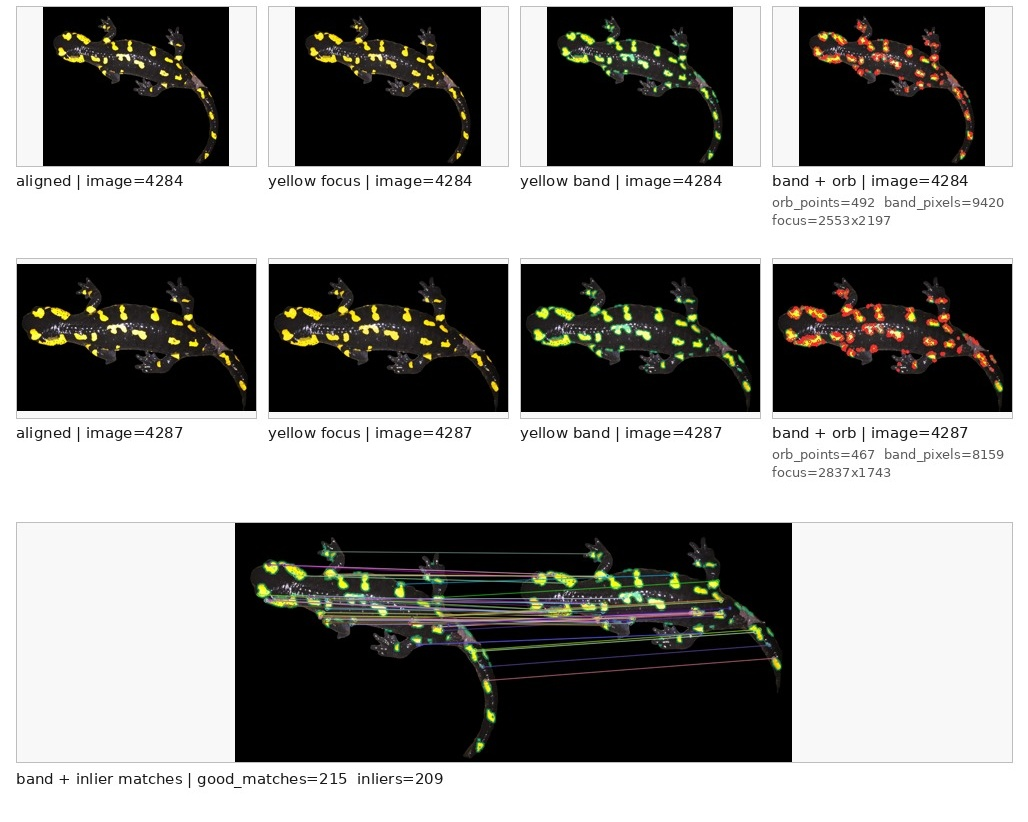
\includegraphics[width=0.92\linewidth]{figures/salamander_yellow_orb_pair.jpg}
  \caption{Yellow-pattern guided local evidence for a salamander candidate pair. The upper rows show aligned views, yellow-focused views, yellow-band views, and ORB keypoints. The bottom panel shows inlier matches after local geometric verification. This illustrates why yellow-pattern information is useful as pairwise evidence but should be consumed by a learned or verified graph stage rather than as a hard global veto.}
  \label{fig:salamander-yellow-orb}
\end{figure}

The final competition gains came from scaling the same idea to higher-recall salamander candidates. The automatic models supplied candidate recall, while pair-constraint verification supplied enough precision to repair the clustering graph through targeted pair evidence.

\subsection{SeaTurtleID2022}
Sea turtle was the most stable branch. Frozen MegaDescriptor+MiewID fusion already reached 0.9256 validation ARI, and supervised routes did not reliably improve it. We therefore kept this branch conservative, adding only a cropped-view fusion branch that improved the public leaderboard from 0.49605 to 0.49726 when applied on top of the current mixed base.

\subsection{TexasHornedLizards}
\dataset{TexasHornedLizards} was released without labelled train images, so the original descriptor fallback was poorly calibrated. Lower-threshold descriptor variants helped, but the first major recovery came from a Texas-specific self-training route, which increased the public leaderboard to 0.45751.

The official Texas horned lizard reference paper by Biffi et al. \cite{biffi2025identification} confirmed that individual identity can be read from ventral spot patterns. In their HotSpotter experiment, the first-ranked candidate was correct for 94.4\% of known recapture photos, while most remaining failures still contained the true match in the top-10 list. This directly shaped our route: use SAM-aligned \cite{sam}, gray-percentile, center-body-square views to expose ventral markings, retrieve inclusive top-$K$ candidates, and then compile trusted candidate links into the clustering graph. Figure~\ref{fig:texas-preprocess-audit} shows the early data-analysis audit that led to this view-normalisation route.

\begin{figure}[t]
  \centering
  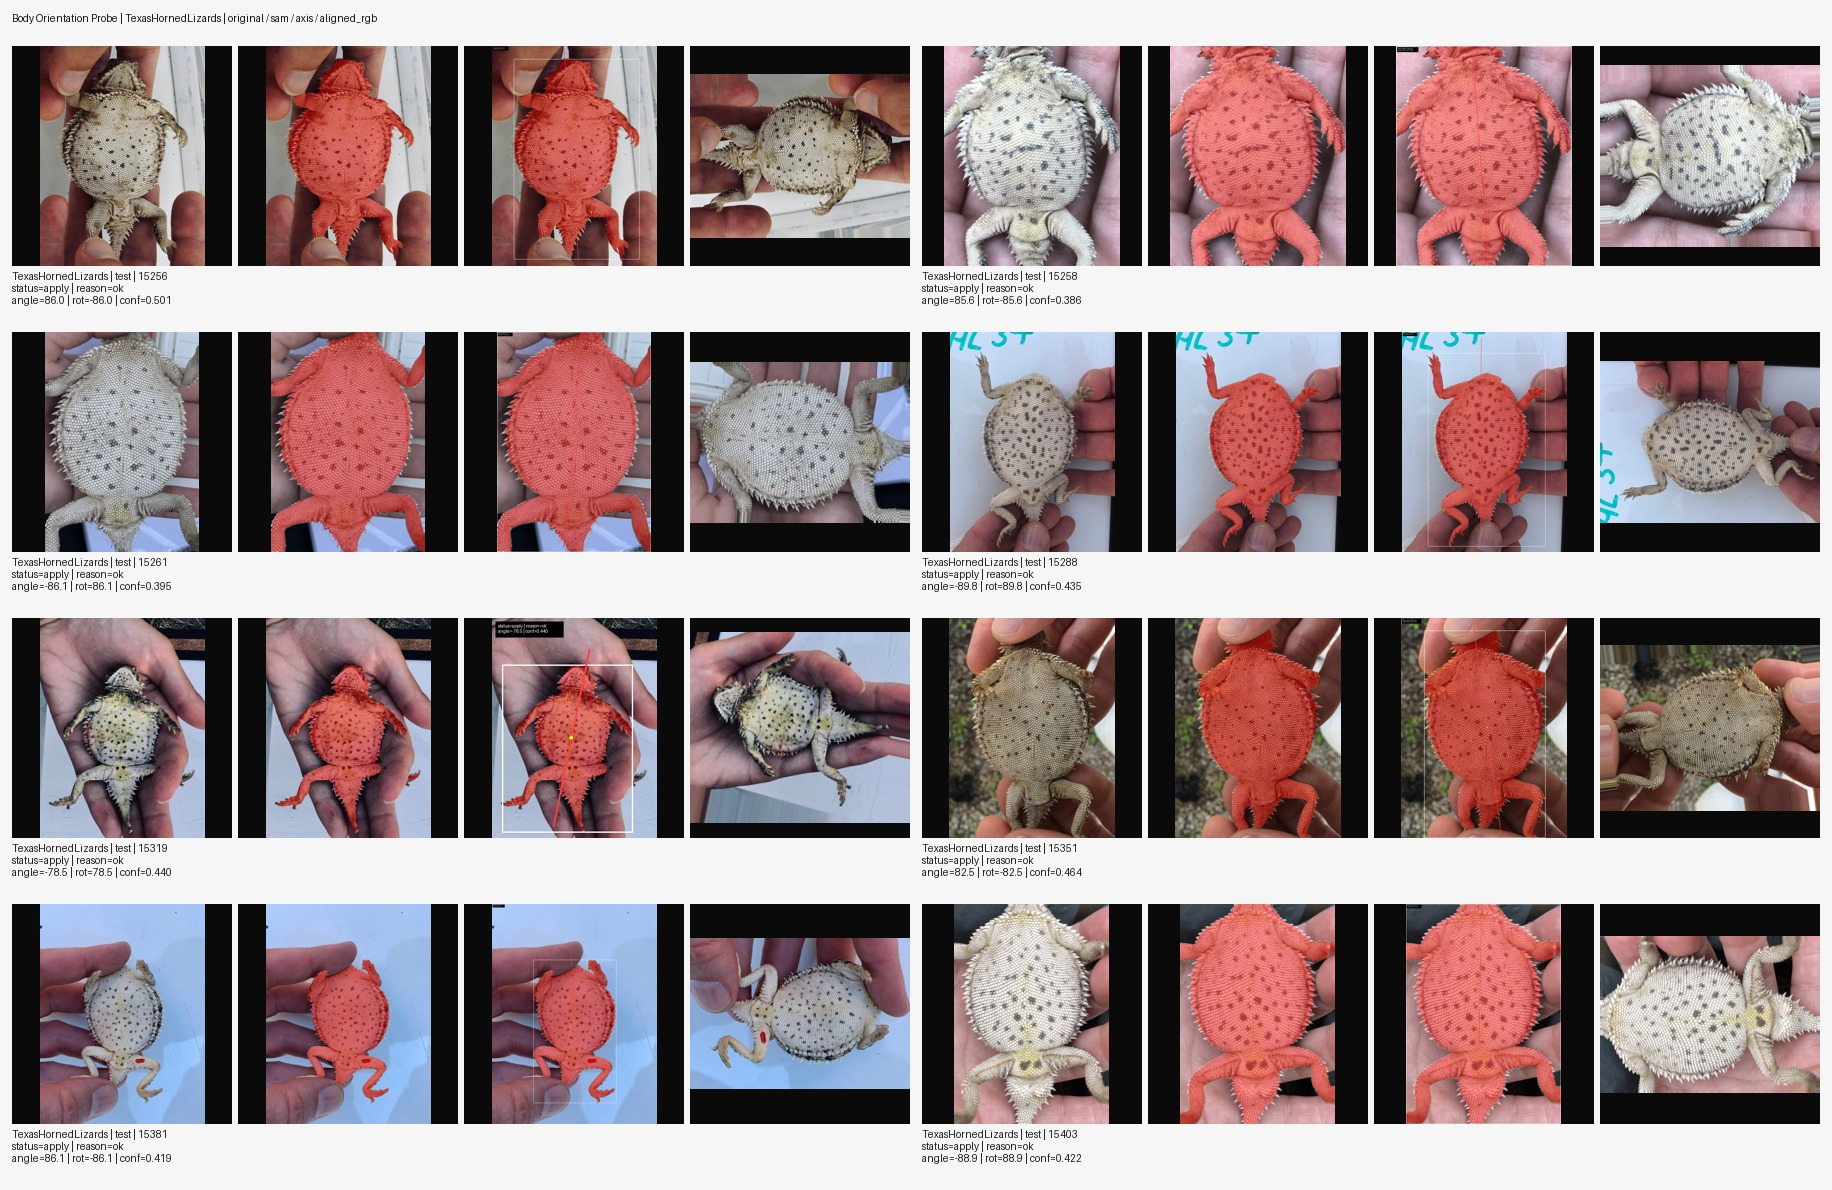
\includegraphics[width=\linewidth]{figures/texas_body_orientation_probe.jpg}
  \caption{Early Texas horned lizard preprocessing audit. Each group compares the original image, segmentation mask, estimated body axis, and aligned body view. The audit showed that ventral spot layouts could be made more comparable by masking and orientation normalisation before local pair matching.}
  \label{fig:texas-preprocess-audit}
\end{figure}

The self-training route used pseudo-labels only after view normalization and conservative candidate filtering. We first constructed SAM-aligned gray center-body views, retrieved top-$K$ neighbours using descriptor and local evidence, and accepted only high-confidence links as trusted pseudo-positive pairs. These pairs, together with single-view consistency positives from all images, produced a small trusted training set for a Texas-specific MiewID student. The remaining bottleneck was graph connectivity: the route needed more reliable positive connections than descriptor thresholding alone could provide. Figure~\ref{fig:texas-orb-pair} shows the kind of local ventral-pattern evidence used by this interface.

\begin{figure}[t]
  \centering
  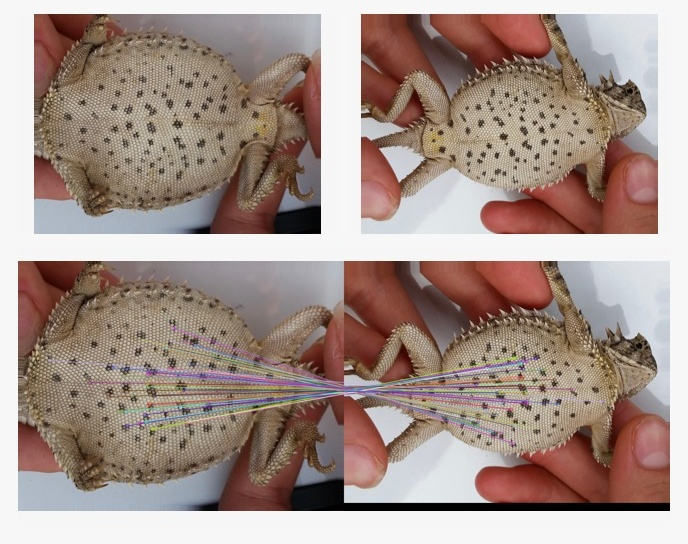
\includegraphics[width=0.82\linewidth]{figures/texas_orb_verified_pair.jpg}
  \caption{Local ventral-pattern evidence for a Texas horned lizard candidate pair. The top row shows two candidate images after view normalization; the bottom row overlays ORB inlier matches on ventral spot patterns. The example motivates using local matching as a high-recall candidate generator followed by pair-constraint verification and trusted graph compilation.}
  \label{fig:texas-orb-pair}
\end{figure}

The final Texas route trained a MiewID-based student using trusted supervision plus all-image single-view pseudo-positive consistency. Replacing only the Texas branch with this trusted-view route increased the public leaderboard from 0.51595 to 0.53646. More importantly, Texas established the pair-constraint principle later reused for salamanders: retrieve high-recall candidate pairs automatically, verify only ambiguous pairs, and compile the trusted decisions into a stronger clustering graph. Additional construction details are given in Appendix~\ref{app:route-details}.

\section{Results and Submission Trace}
The empirical story is that the pipeline moved from automatic dataset-routed clustering to graph-constrained candidate-pair repair. Before pair-constraint verification, the public-best routed base reached 0.51595 public ARI with supervised/frozen descriptors, salamander ORB and XGBoost fusion, yellow-pattern features, sea-turtle crop fusion, lynx seed smoothing, and conservative constraint compilation. After scaling pair-constraint verification to Texas and salamander, the final submission reached 0.67987 public ARI and 0.69632 private ARI.

Table~\ref{tab:public-progress} summarizes the documented intervention trace. It is an engineering trace rather than a controlled factorial ablation, but it identifies the stages that produced the largest visible changes.

\begin{table}[t]
  \centering
  \caption{Submission trace by intervention stage. Scores are ARI.}
  \label{tab:public-progress}
  \small
  \begin{tabularx}{\linewidth}{lrrY}
    \toprule
    Stage & Public ARI & Private ARI & Main change \\
    \midrule
    Data-routed base & 0.372 & -- & Lynx used MegaDescriptor fine-tuning; salamander used Miew/Mega fusion plus ORB-enhanced clustering; sea turtle used frozen MegaDescriptor+MiewID fusion; Texas used unsupervised descriptor clustering. \\
    Texas self-training & 0.457 & -- & SAM-aligned Texas views, high-confidence top-$K$ pseudo-positive links, and a Texas-specific MiewID student. \\
    Salamander XGBoost fusion & 0.485 & -- & Learned pairwise fusion over global similarities, branch-score differences, ORB score, inliers, and match ratios. \\
    Yellow-ROI local evidence & 0.515 & -- & Colour-based yellow ROIs focused salamander local evidence before ORB-based matching features were fused. \\
    Public-best routed base before pair constraints & 0.51595 & 0.44839 & Automatic routed clustering with learned pairwise fusion and conservative constraint compilation. \\
    Private-best observed base before pair constraints & 0.48835 & 0.46575 & Post-hoc reference from the Kaggle export after private scores were released. \\
    Final pair constraints & 0.67987 & 0.69632 & Texas trusted-view self-training plus salamander top-$K$ pair verification and positive graph constraints. \\
    \bottomrule
  \end{tabularx}
\end{table}

The two before-verification rows use different selection rules: the public-best base was the development anchor during the competition, while the private-best observed base is only a post-hoc reference. Additional cluster-shape diagnostics and negative probes are reported in Appendix~\ref{app:additional-results}.

\section{Discussion}
The main observation is that AnimalCLEF 2026 is not only a representation-learning task. It is a partitioning problem under species-specific evidence, long-tailed identities, open-set test clusters, and incomplete local supervision. We found that strong pretrained descriptors were necessary but not sufficient. The most valuable work happened after candidate retrieval: deciding which pair evidence was trustworthy, which dataset should receive local matching, how to calibrate thresholds, and how to keep local validation evidence separate from official leaderboard observations.

Another lesson is that a test-only clustering graph can have an insufficient information budget for some individuals. A single weak view may not expose enough distinctive markings to decide a merge or split, so the useful route is often to expose better identity evidence before clustering. Sea turtle benefited from cropped-view fusion, Texas horned lizards from SAM-aligned body views, and salamanders from local yellow-pattern pair evidence.

The pair verification component deserves careful framing. It was restricted to model-selected candidate pairs and ambiguous clusters, then compiled into deterministic split and graph-constraint operations. The decisions were pair-level constraints over visible image evidence, not hidden labels or direct identity assignments. This made the constraints reproducible and inspectable. In Texas, the pair-verification loop first produced trusted pair evidence and then a stronger self-training set. In salamander, the same idea was reused mainly as ambiguity-zone pair verification and constraint compilation.

The largest limitation of this note is that it records a competition pipeline whose final branch selection depended on public leaderboard feedback and many local artifacts. We therefore report leaderboard gains mainly as intervention-level evidence. For reproducibility, this note reports the branch-level preprocessing, model choices, thresholds, and graph-compilation settings used by the submitted pipeline. The final submitted CSV was uploaded on 2026-04-29 03:04:38 UTC and is associated with the public/private scores reported in Table~\ref{tab:public-progress}.

\section{Conclusion}
We presented a dataset-routed hybrid clustering pipeline for AnimalCLEF 2026 that obtained 0.67987 public ARI and 0.69632 private ARI. The central lesson is that this benchmark was not solved by a single embedding or threshold. Performance improved when each dataset exposed its own identity evidence and when uncertain retrieval links were converted into graph constraints. For lynx and sea turtles, conservative descriptor clustering was sufficient; for salamanders and Texas horned lizards, local candidate-pair evidence and constraint compilation were the decisive parts of the final pipeline.

\begin{acknowledgments}
We thank the AnimalCLEF 2026 organizers for preparing the benchmark, maintaining the Kaggle competition, and providing the evaluation infrastructure. We also thank the maintainers and authors of the open-source animal re-identification resources and pretrained models used in this work, including MiewID, MegaDescriptor, WildlifeDatasets, scikit-learn, OpenCV, and XGBoost.
\end{acknowledgments}

\section*{Declaration on Generative AI}
During the preparation of this work, the authors used generative AI tools for coding assistance, experiment organization, and language editing. The method design, experiments, result interpretation, and final manuscript content were reviewed and are the responsibility of the authors.

\appendix
\section{Implementation Details}
\label{app:implementation-details}
\begin{table}[h]
  \centering
  \caption{Main branch configuration for the best documented public pipeline.}
  \label{tab:route-config}
  \small
  \begin{tabularx}{\linewidth}{lYrl}
    \toprule
    Dataset & Route & Dim. & Threshold \\
    \midrule
    \dataset{LynxID2025} & MegaDescriptor-L supervised student with seed smoothing / route co-association variants & 512 & 0.8--0.85 \\
    \dataset{SalamanderID2025} & Miew masked-SupCon student + frozen fusion + ORB/XGBoost/yellow features + graph constraints & 4200 & 0.25 \\
    \dataset{SeaTurtleID2022} & frozen MegaDescriptor+MiewID fusion with cropped fusion branch, weight 0.3 & 7376 & 0.7 \\
    \dataset{TexasHornedLizards} & Miew trusted-view self-training on SAM-aligned gray center-body views & 512 & 0.44 \\
    \bottomrule
  \end{tabularx}
\end{table}

\begin{table}[h]
  \centering
  \caption{Key operating parameters of the submitted pipeline. Thresholds are cosine-distance clustering thresholds unless noted otherwise.}
  \label{tab:key-params}
  \small
  \begin{tabularx}{\linewidth}{lYlY}
    \toprule
    Dataset & Main evidence & Gate & Pair-constraint role \\
    \midrule
    \dataset{LynxID2025} & MegaDescriptor supervised student, TTA variants, transductive seed smoothing & 0.8--0.85 & not used; descriptor graph was sufficient \\
    \dataset{SalamanderID2025} & Miew supervised student, frozen fusion, ORB top-$K=10$, yellow-pattern features, XGBoost pair fusion & graph 0.25; ORB inliers $\geq$8 & positive/negative constraints for ambiguous candidates \\
    \dataset{SeaTurtleID2022} & frozen MegaDescriptor+MiewID fusion plus cropped-view fusion with weight 0.3 & 0.7 & not used; conservative descriptor fusion was selected \\
    \dataset{TexasHornedLizards} & SAM-aligned gray center-body views, Miew trusted-view self-training, ORB candidate evidence & 0.44 & automatic trusted pairs first; later pair review for ambiguous candidates \\
    \bottomrule
  \end{tabularx}
\end{table}

MegaDescriptor-L takes 384$\times$384 RGB inputs and outputs a 1536-dimensional vector. MiewID-msv3 takes 440$\times$440 RGB inputs and outputs a 2152-dimensional vector. Early fusion concatenates the two normalised blocks into a 3688-dimensional vector and normalises the result again. For supervised routes, each student backbone is followed by a linear projection to a 512-dimensional L2-normalised embedding. Training uses separate ArcFace heads \cite{arcface} for each dataset rather than one shared closed-set head. We also evaluated feature distillation, relation distillation, masked supervised contrastive loss \cite{supcon}, and a salamander sub-center ArcFace head \cite{arcface}.

ORB extraction used up to 1024 features per image after resizing the longer side to 768 pixels. Candidate matching was implemented with OpenCV \cite{opencv} using brute-force descriptor matching, a ratio test of 0.8, and RANSAC geometric verification \cite{ransac}; pairs with fewer than 8 inliers received zero local support. The local score was used as a conservative boost:
\begin{equation}
  s_{\mathrm{rerank}} = s_{\mathrm{global}} + w_{\mathrm{local}} s_{\mathrm{local}} (1 - s_{\mathrm{global}}).
\end{equation}
Here $s_{\mathrm{global}}$ is the descriptor cosine similarity, $s_{\mathrm{local}}$ is the normalized ORB/RANSAC local evidence, and $w_{\mathrm{local}}$ controls how strongly local matches can boost a pair; the factor $(1-s_{\mathrm{global}})$ keeps the boost small for pairs that are already globally similar.
In the salamander smoke audit, positive pairs had mean local score 0.3366, while negative pairs had mean local score 0.0111.

For the gate2 salamander compiler, we used \method{graph\_threshold=0.25}, \method{min\_judged\_pairs=2}, and \method{min\_no\_pairs=2}. The gate compiled 42 candidates, skipped 61 low-evidence candidates, changed 89 salamander images, and produced 60 overlay operations. Compared with a split-only base, it reduced salamander clusters from 427 to 412 and singletons from 260 to 229.

\section{Additional Route Details}
\label{app:route-details}
For lynx, we also tested route co-association over multiple supervised routes and thresholds. The useful variants combined synth-warmup and previous-best TTA routes through average, mutual-$k$NN, and complete-link style predictions, then kept pairs supported by a high co-association vote threshold. These probes were secondary to the final pipeline because the lynx branch was already reasonably stable under supervised metric learning and seed smoothing.

For salamanders, the final route was built in five stages: frozen MegaDescriptor+MiewID fusion; ORB local reranking only for salamanders; a MiewID-based supervised embedding trained with masked supervised contrastive loss and concatenated with frozen fusion features; XGBoost pairwise fusion over global, local, and route-specific features; and split or pair-constraint judgments compiled into a graph overlay. A yellow-only veto looked plausible because this dataset is dominated by yellow dorsal markings, but it over-fragmented clusters and reduced local validation ARI from 0.5875 to 0.2905 in one probe. The same cue, when introduced as an XGBoost feature, improved the public leaderboard from 0.49726 to 0.51082.

For Texas horned lizards, the trusted-view student used 46 trusted images and 228 untrusted images, producing 1142 training rows after view construction. The final selected route used trusted supervision plus all-image single-view pseudo-positive consistency, without teacher distillation. The branch was valuable not only for its own leaderboard gain but also because it established the top-$K$ candidate retrieval and pair-verification interface later reused on salamanders.

\section{Additional Results and Probes}
\label{app:additional-results}
\begin{table}[h]
  \centering
  \caption{Cluster shape of the best documented public submission after Texas trusted-view self-training.}
  \label{tab:cluster-shape}
  \begin{tabular}{lrrrr}
    \toprule
    Dataset & Samples & Clusters & Singleton clusters & Singleton ratio \\
    \midrule
    \dataset{LynxID2025} & 946 & 43 & 5 & 0.116 \\
    \dataset{SalamanderID2025} & 689 & 423 & 257 & 0.608 \\
    \dataset{SeaTurtleID2022} & 500 & 153 & 41 & 0.268 \\
    \dataset{TexasHornedLizards} & 274 & 242 & 220 & 0.909 \\
    \bottomrule
  \end{tabular}
\end{table}

Several negative results shaped the final pipeline. Descriptor concatenation for Texas preserved high-confidence seed pairs but degraded the public score, suggesting that the proxy did not penalise outsider merges near seed clusters. Salamander yellow cues were harmful as hard vetoes but helpful as learned pairwise features. Deep local matching probes with ALIKED \cite{aliked} and LightGlue \cite{lightglue}, plus a WildFusion-style calibration, did not outperform the simpler ORB-based route in our validation protocol. Dual-view SAM-masked salamander routes were engineering-ready but did not improve official submissions when directly inserted into the current XGBoost pipeline.

\bibliography{references}

\end{document}
